\documentclass{article}
\PassOptionsToPackage{numbers, compress}{natbib}
\usepackage[final]{nips_2017}
\usepackage[utf8]{inputenc}
\usepackage[T1]{fontenc}
\usepackage{hyperref}
\usepackage{url}
\usepackage{nicefrac}
\usepackage{microtype}
\usepackage{amsmath,amssymb,amsfonts}
\usepackage{graphicx}
\usepackage{textcomp}
\usepackage{xcolor}
\usepackage{booktabs}
\usepackage{setspace}
\usepackage{subcaption}

\def\BibTeX{{\rm B\kern-.05em{\sc i\kern-.025em b}\kern-.08em
    T\kern-.1667em\lower.7ex\hbox{E}\kern-.125emX}}

\begin{document}

\title{Optimized Contrastive Deep Nonnegative Matrix Factorization for Community Detection}

\author{
  Longjie Ran \\
  School of Information Science and Technology \\
  ShanghaiTech University \\
  Shanghai, China \\
  \texttt{ranlj2025@shanghaitech.edu.cn}
}

\maketitle

\begin{abstract}
Community detection is a fundamental task in network analysis that requires the effective integration of topological structure and node attributes. Although Contrastive Deep Nonnegative Matrix Factorization (CDNMF) has emerged as a powerful framework for this purpose, its standard implementation suffers from computational bottlenecks—specifically $O(N^2)$ complexity—and relies on a simplistic multi-view fusion strategy. In this paper, we present a comprehensive optimization of CDNMF that addresses these scalability and performance limitations. We mathematically reformulate the reconstruction and regularization objectives to exploit matrix sparsity, reducing the computational complexity to $O(E + Nk)$. To better synthesize information from diverse views, we introduce an adaptive attention-based fusion mechanism, complemented by Dropout regularization to enhance generalization. Furthermore, we establish a robust AutoML pipeline using Optuna for automated hyperparameter tuning. Extensive experiments on benchmark datasets demonstrate that our optimized model achieves a 2.6$\times$ speedup on PubMed, while significantly outperforming the baseline with accuracy improvements of up to 13.57\% on the PubMed dataset.
\end{abstract}

\section{Introduction}
The exponential growth of real-world networks, including social media platforms, citation networks, and biological interaction graphs, has necessitated the development of efficient algorithms for analyzing their underlying structure. Community detection, also known as graph clustering, is a fundamental task in this domain that serves as a building block for applications ranging from recommendation systems to functional module identification in protein-protein interaction networks.

Traditional methods, such as spectral clustering and modularity maximization, primarily focus on the topological structure of the graph. However, real-world graphs often contain rich node attributes (e.g., textual content in citation networks, user profiles in social networks) that complement the topology. Integrating these two sources of information is essential for improving detection performance.

Nonnegative Matrix Factorization (NMF) \cite{lee1999learning} has emerged as a powerful technique for community detection. Unlike spectral methods that can produce negative values, NMF enforces non-negativity constraints, yielding additive, part-based representations that are readily interpretable as community memberships. To capture complex hierarchical structures in data, Deep NMF \cite{trigeorgis2017deep} extends standard NMF by stacking multiple factorization layers, thereby learning high-level features.

Despite these advancements, standard Deep NMF methods often treat topology and attributes separately or fuse them in a naive manner. Contrastive Deep Nonnegative Matrix Factorization (CDNMF) \cite{li2024contrastive} addresses these issues by introducing contrastive learning to align community membership representations derived from network topology and node attributes. By maximizing the similarity between representations of the same node from different views (positive pairs) and minimizing it for different nodes (negative pairs), CDNMF learns a more robust consensus representation.

Although the conceptual framework of CDNMF is sound, its standard implementation faces severe scalability challenges. The algorithm typically involves computing dense similarity matrices and reconstruction errors that scale quadratically with the number of nodes $N$. For large-scale graphs with millions of nodes, this $O(N^2)$ complexity is prohibitive. Furthermore, the fusion of structural and attribute representations is often performed via simple averaging, which fails to account for the varying informativeness of the two views across different nodes.

In this paper, we present a comprehensive optimization of the CDNMF framework. Our contributions are fourfold:
\begin{itemize}
    \item \textbf{Sparse Optimization:} We derive a mathematically equivalent reformulation of the reconstruction and regularization loss functions that avoids constructing $N \times N$ dense matrices, thereby reducing the computational complexity from $O(N^2)$ to $O(E + Nk)$, where $E$ is the number of edges and $k$ is the latent dimension.
    \item \textbf{Attention-based Fusion:} We replace the static averaging fusion strategy with a learnable attention mechanism that dynamically assigns weights to the structural and attribute views.
    \item \textbf{Dropout Regularization:} We incorporate Dropout layers within the Deep NMF modules to prevent overfitting and improve the generalization capability of the model.
    \item \textbf{AutoML Integration:} We design a decoupled pre-training and fine-tuning workflow using Optuna \cite{akiba2019optuna}, enabling efficient and automated hyperparameter optimization.
\end{itemize}

The remainder of this paper is organized as follows: Section~II provides an overview of the existing CDNMF framework. Section~III critiques the limitations of the current state-of-the-art. Section~IV details our proposed optimizations and contributions. Section~V presents numerical results validating our approach. Finally, Section~VI concludes the paper.

\section{Overview of Existing Work}

\subsection{Problem Formulation}
We consider an attributed graph $G=(V, E, X)$, where $V$ is the set of $N$ nodes, $E$ is the set of edges, and $X \in \mathbb{R}^{N \times F}$ is the node attribute matrix with $F$ features per node. The graph structure is represented by an adjacency matrix $A \in \mathbb{R}^{N \times N}$. The goal of community detection is to partition the nodes into $K$ disjoint groups. In the context of NMF, this corresponds to learning a non-negative community membership matrix $H \in \mathbb{R}^{N \times K}$, where $H_{ik}$ indicates the degree to which node $i$ belongs to community $k$.

\subsection{Deep NMF}
Standard NMF approximates a non-negative matrix $M$ as the product of two low-rank non-negative matrices $W$ and $H^T$. Deep NMF extends this formulation by decomposing the matrix into multiple layers:
\begin{equation}
    M \approx W_1 W_2 \cdots W_m H^T
\end{equation}
where $W_i$ denotes the mapping matrix for each layer and $H$ is the final representation. This multi-layer structure enables the model to learn a hierarchy of features, mapping the high-dimensional input space to a low-dimensional community space.

\subsection{The CDNMF Model}
The CDNMF model \cite{li2024contrastive} employs a dual-pathway architecture to process topology and attributes simultaneously:

\begin{figure}[htbp]
    \centering
    \includegraphics[width=0.8\linewidth]{../picture/image.png}
    \caption{Overview of the CDNMF model architecture.}
    \label{fig:cdnmf_overview}
\end{figure}

\begin{enumerate}
    \item \textbf{Structure View:} A Deep NMF module factorizes the adjacency matrix $A$:
    \begin{equation}
        A \approx U_{net}^{(1)} \dots U_{net}^{(m)} (V_{net})^T
    \end{equation}
    \item \textbf{Attribute View:} A separate Deep NMF module factorizes the attribute matrix $X^T$:
    \begin{equation}
        X^T \approx U_{att}^{(1)} \dots U_{att}^{(m)} (V_{att})^T
    \end{equation}
\end{enumerate}

The overall objective function is a weighted sum of four components:
\begin{equation}
    \mathcal{L} = \mathcal{L}_{rec} + \alpha \mathcal{L}_{con} + \beta \mathcal{L}_{reg} + \gamma \mathcal{L}_{neg}
\end{equation}

\subsubsection{Reconstruction Loss ($\mathcal{L}_{rec}$)}
This term ensures that the learned representations faithfully reconstruct the original input data. It is defined as the sum of squared Frobenius norms of the reconstruction errors for both views:
\begin{equation}
    \mathcal{L}_{rec} = \|A - \hat{A}\|_F^2 + \|X^T - \hat{X}\|_F^2
\end{equation}
where $\hat{A}$ and $\hat{X}$ are the reconstructed matrices from the Deep NMF layers.

\subsubsection{Contrastive Loss ($\mathcal{L}_{con}$)}
To align the representations from the two views, CDNMF employs a contrastive loss. This loss treats representations of the same node from the two views ($v_{net, i}$ and $v_{att, i}$) as a positive pair and representations of different nodes as negative pairs. The objective encourages high similarity for positive pairs and low similarity for negative pairs, typically using a formulation similar to InfoNCE or a semi-supervised variant that leverages pseudo-labels.

\subsubsection{Regularization ($\mathcal{L}_{reg}$)}
To incorporate the geometric structure of the data, a graph regularization term is commonly added. This term assumes that connected nodes should have similar representations and is typically formulated using the graph Laplacian $L = D - A$:
\begin{equation}
    \mathcal{L}_{reg} = \text{Tr}(V_{net} L V_{net}^T) + \text{Tr}(V_{att} L V_{att}^T)
\end{equation}
Minimizing this term enforces smoothness of the representation on the graph manifold.

\section{Criticism of Existing Works}

Although CDNMF represents a significant advancement by integrating contrastive learning with NMF, a critical analysis reveals several limitations in its standard formulation and implementation.

\subsection{Computational Inefficiency and Scalability}
The most significant limitation is the computational complexity associated with the reconstruction loss. The term $\|A - \hat{A}\|_F^2$ involves the difference between the sparse adjacency matrix $A$ and the dense reconstructed matrix $\hat{A} = WH^T$.
\begin{itemize}
    \item \textbf{Memory Complexity:} Storing the dense matrix $\hat{A}$ requires $O(N^2)$ memory. For a moderately sized graph such as PubMed ($N \approx 20,000$), a float32 matrix requires $20000^2 \times 4$ bytes $\approx 1.6$ GB. For a larger graph with 100,000 nodes, this would require 40 GB, exceeding the memory capacity of most GPUs.
    \item \textbf{Time Complexity:} Computing the Frobenius norm of an $N \times N$ matrix requires $O(N^2)$ operations, rendering the training process prohibitively slow for large graphs.
\end{itemize}
Similarly, the regularization term $\text{Tr}(H L H^T)$ often involves constructing the dense Laplacian matrix or performing dense matrix multiplications, further hindering scalability.

\subsection{Naive Fusion Strategy}
The original CDNMF model typically fuses the representations from the structural and attribute views using a simple linear combination, such as averaging: $H = 0.5 H_{net} + 0.5 H_{att}$. This strategy relies on the strong assumption that both views are equally reliable and informative for every node in the graph. However, in practice, this assumption rarely holds. Some nodes may possess rich textual attributes but sparse connections (making the attribute view more informative), while others may be well-connected but lack descriptive attributes (making the structural view more informative). A static, global fusion weight fails to capture these node-level variations.

\subsection{Lack of Modern Regularization Techniques}
Deep NMF models, similar to other deep neural networks, are susceptible to overfitting, particularly when the number of parameters is large relative to the dataset size. The original implementation relies primarily on graph regularization and lacks modern regularization techniques commonly employed in deep learning, such as Dropout, which randomly deactivates units during training to prevent co-adaptation and improve generalization.

\section{New Contributions}

To address the aforementioned limitations, we propose a series of optimizations and architectural enhancements.

\subsection{Mathematical Optimization for Sparse Computation}
We reformulate the loss functions to exploit the sparsity of the adjacency matrix $A$, reducing the complexity from quadratic to linear in the number of nodes and edges.

\subsubsection{Optimized Reconstruction Loss}
Instead of computing the norm of the difference matrix directly, we expand the squared Frobenius norm:
\begin{equation}
    \|A - WH^T\|_F^2 = \text{Tr}((A - WH^T)^T (A - WH^T))
\end{equation}
\begin{equation}
    = \text{Tr}(A^T A) + \text{Tr}((WH^T)^T WH^T) - 2\text{Tr}(A^T WH^T)
\end{equation}
We analyze each term separately:
\begin{itemize}
    \item $\text{Tr}(A^T A) = \|A\|_F^2$: This is a constant scalar that can be precomputed once.
    \item $\text{Tr}((WH^T)^T WH^T) = \text{Tr}(H H^T W^T W)$: By computing the smaller matrices $H H^T$ ($K \times K$) and $W^T W$ ($K \times K$) first, this term can be evaluated in $O(NK^2)$ time, which is linear in $N$.
    \item $\text{Tr}(A^T WH^T) = \text{Tr}(H^T (AW))$: Since $A$ is sparse, the product $AW$ can be computed using sparse matrix multiplication in $O(EK)$ time. The subsequent trace operation requires $O(NK)$.
\end{itemize}
By implementing this reformulation, we avoid constructing any $N \times N$ dense matrix. The total complexity becomes $O(E + NK^2)$, which is significantly more efficient than $O(N^2)$.

\begin{figure}[htbp]
    \centering
    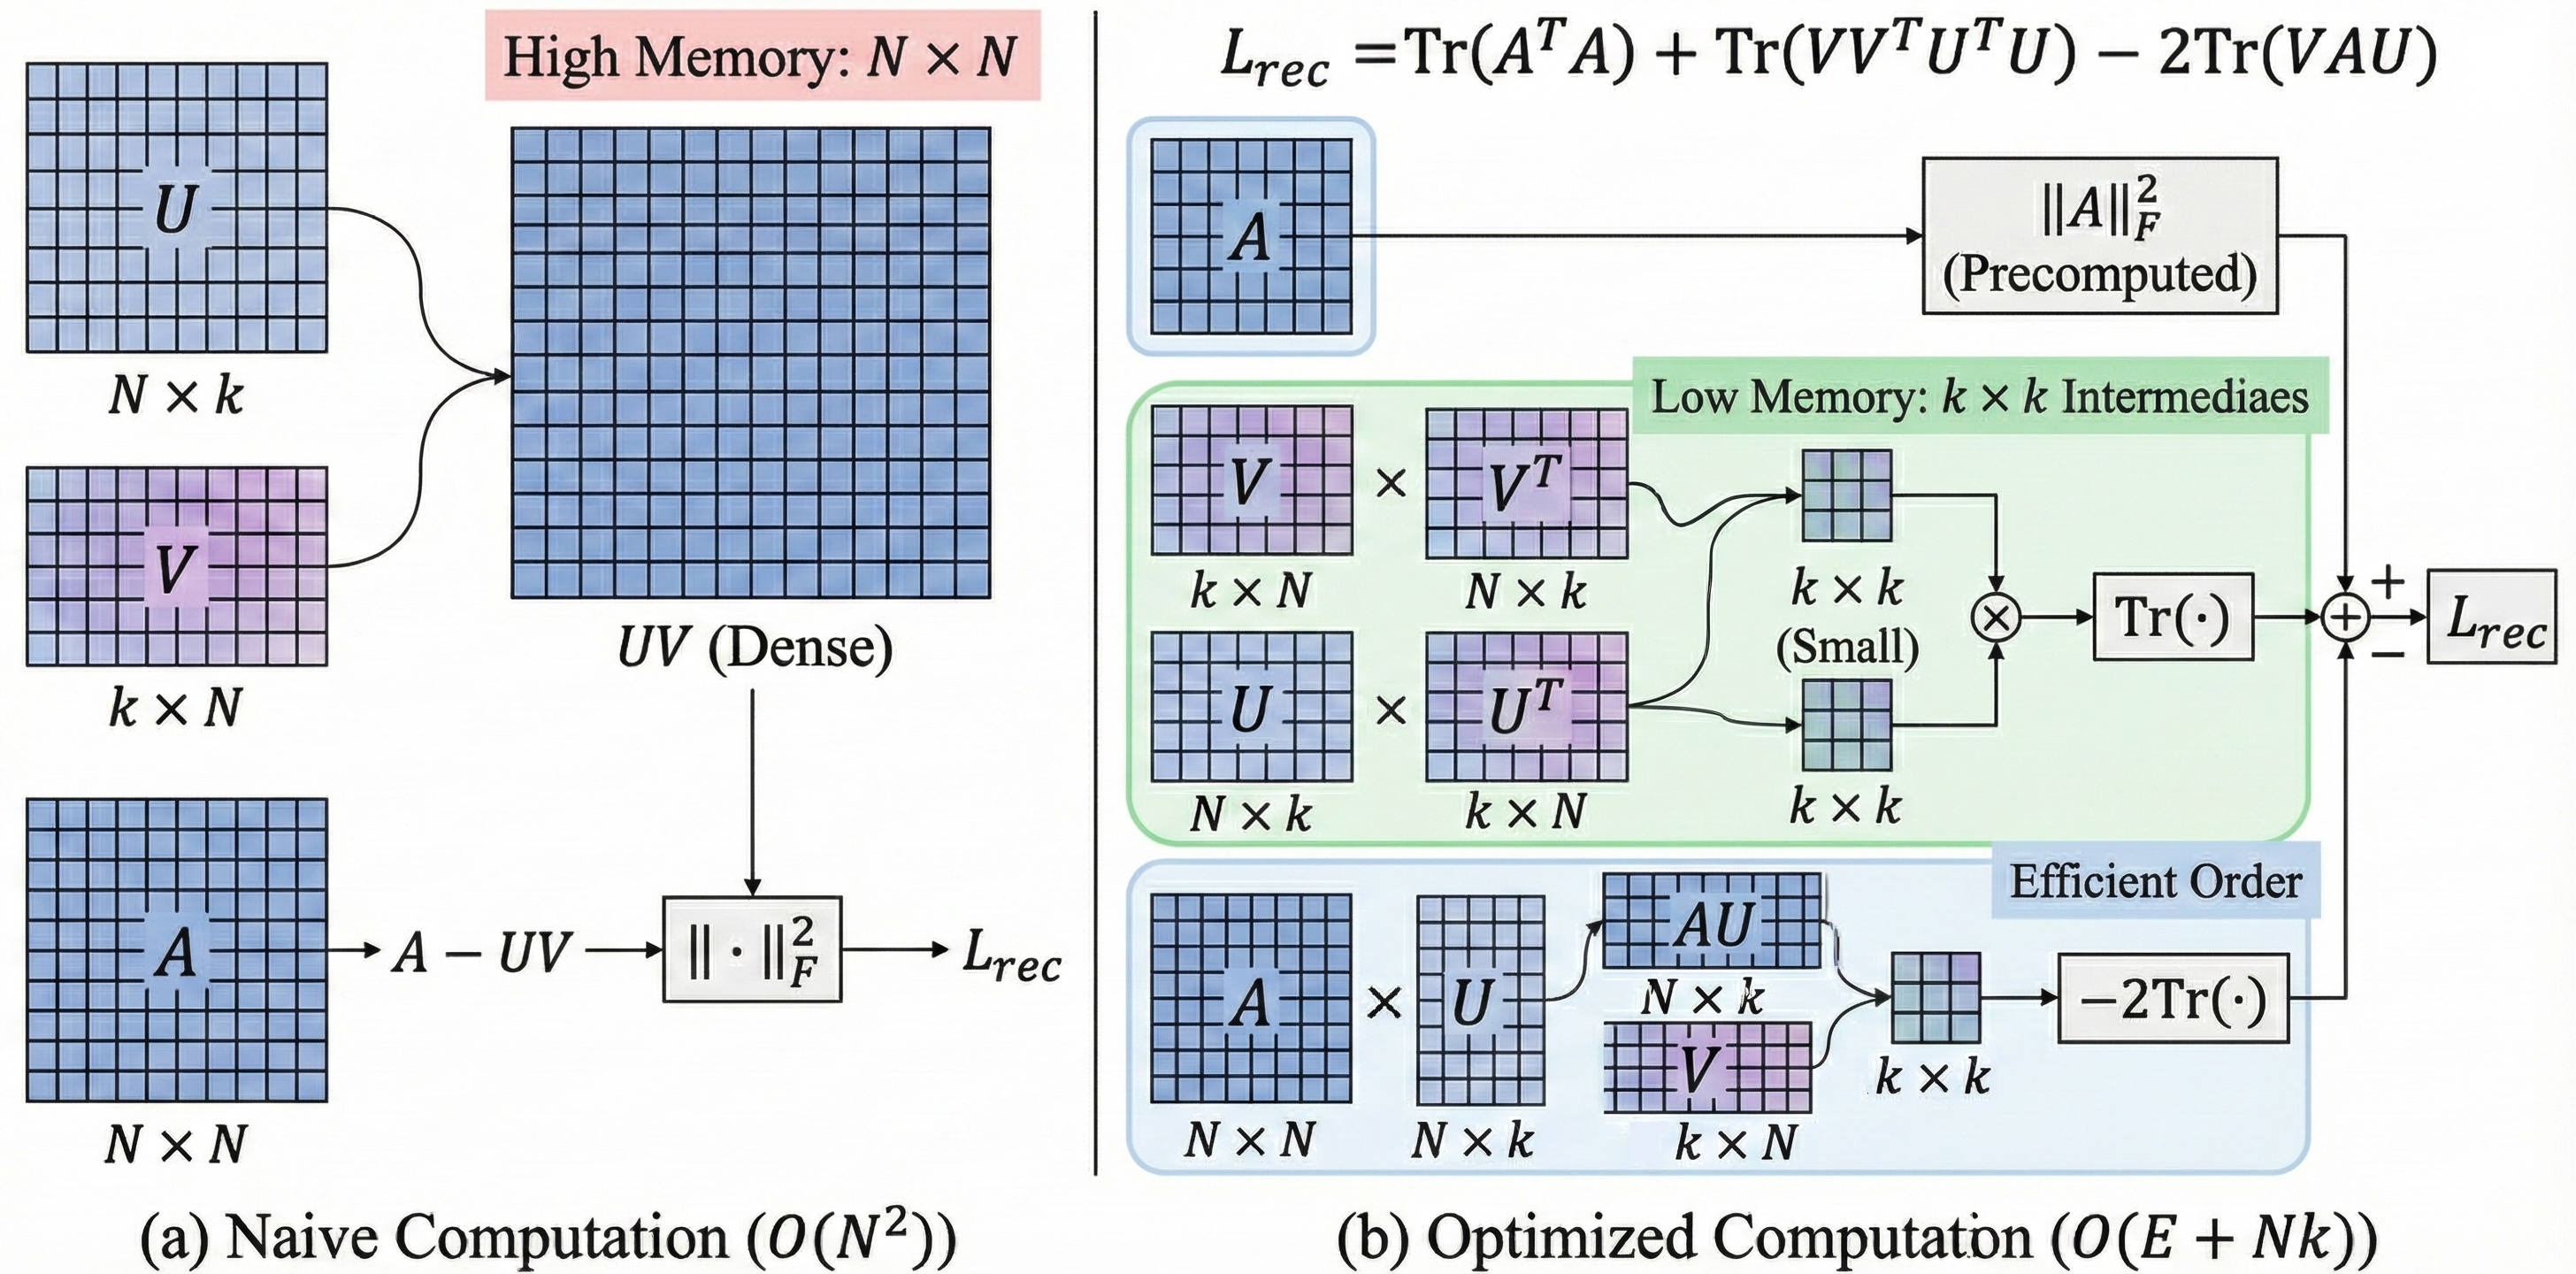
\includegraphics[width=0.8\linewidth]{../picture/4.1.1 Optimized Reconstruction Loss.png}
    \caption{Illustration of the optimized reconstruction loss calculation avoiding dense matrix construction.}
    \label{fig:opt_loss}
\end{figure}

\subsubsection{Optimized Regularization Loss}
Similarly, we optimize the graph regularization term $\text{Tr}(H L H^T)$. Using the definition $L = D - A$:
\begin{equation}
    \text{Tr}(H (D-A) H^T) = \text{Tr}(H D H^T) - \text{Tr}(H A H^T)
\end{equation}
\begin{itemize}
    \item $\text{Tr}(H D H^T) = \sum_j D_{jj} \|H_{:j}\|^2$: Since $D$ is diagonal, this term can be computed using element-wise vector operations in $O(NK)$.
    \item $\text{Tr}(H A H^T)$: This term can be computed efficiently using sparse matrix multiplication for $A$, analogous to the reconstruction loss.
\end{itemize}

\subsection{Attention-based Fusion}
To enable adaptive integration of the two views, we introduce a learnable attention-based fusion layer. Let $h_{net, i}$ and $h_{att, i}$ denote the learned representations for node $i$ from the structural and attribute branches, respectively. We concatenate these representations and pass them through a fully connected layer followed by a sigmoid activation to compute a fusion weight $\alpha_i \in [0, 1]$:
\begin{equation}
    \alpha_i = \sigma(W_{fusion} [h_{net, i} \| h_{att, i}] + b_{fusion})
\end{equation}


\begin{figure}[htbp]
    \centering
    \includegraphics[width=0.8\linewidth]{../picture/Fusion+dropout.jpg}
    \caption{The proposed architecture incorporating Attention-based Fusion and Dropout Regularization.}
    \label{fig:fusion_dropout}
\end{figure}

The final fused representation is computed as a weighted sum:
\begin{equation}
    h_{fused, i} = \alpha_i \cdot h_{net, i} + (1-\alpha_i) \cdot h_{att, i}
\end{equation}

This mechanism enables the model to adaptively weight the more informative view for each individual node, thereby improving the quality of the final community assignments.


\subsection{Dropout Regularization}
Deep NMF models, despite their matrix factorization origins, are essentially deep neural networks and are thus susceptible to overfitting. The original CDNMF model relies solely on graph regularization. We introduce Dropout layers between the factorization layers, where during training, each element of the latent representation is zeroed out with probability $p$ (a hyperparameter tuned via Optuna). This mechanism forces the network to learn redundant representations and prevents co-adaptation of features, resulting in more robust community detection performance on unseen data and noisy graphs.



\subsection{AutoML Workflow with Optuna}
Hyperparameter tuning constitutes a major bottleneck in Deep NMF research. We implement a decoupled workflow to accelerate this process:
\begin{enumerate}
    \item \textbf{Pre-training Cache:} We pre-train the encoder layers for various architectural configurations (e.g., different hidden layer sizes) and save the parameters to disk. This represents a one-time computational cost.
    \item \textbf{Efficient Search:} We employ Optuna to search for optimal hyperparameters (learning rate, regularization coefficients, and fusion weights). The search script loads the pre-trained parameters from the cache instead of retraining from scratch for each trial, reducing the time per trial from minutes to seconds and enabling exploration of a substantially larger search space.
\end{enumerate}

\begin{figure}[htbp]
    \centering
    \includegraphics[width=0.8\linewidth]{../picture/optuna.jpg}
    \caption{The decoupled AutoML workflow using Optuna for efficient hyperparameter search.}
    \label{fig:optuna}
\end{figure}

\section{Numerical Results}

We evaluated the proposed optimized CDNMF on three standard citation network datasets: Cora, Citeseer, and PubMed. We compared our model against several state-of-the-art baselines in terms of community detection performance (Accuracy and NMI) and computational efficiency (training time and memory usage).


\subsection{Community Detection Performance}
We compared our method against various baselines, including traditional NMF variants, graph embedding methods, and recent deep learning approaches. The results are summarized in Table~\ref{tab:performance}.
\begin{table}[htbp]
    \centering
    \caption{Community detection performance (ACC and NMI) on three datasets.}
    \label{tab:performance}
    \begin{tabular}{lcccccc}
        \toprule
         & \multicolumn{2}{c}{Cora} & \multicolumn{2}{c}{Citeseer} & \multicolumn{2}{c}{PubMed} \\
        \cmidrule(lr){2-3} \cmidrule(lr){4-5} \cmidrule(lr){6-7}
        Method & ACC & NMI & ACC & NMI & ACC & NMI \\
        \midrule
        NMF & 0.4103 & 0.2851 & 0.3074 & 0.1319 & 0.5133 & 0.1606 \\
        ONMF & 0.3811 & 0.2416 & 0.3330 & 0.1423 & 0.5575 & 0.1582 \\
        BNMF & 0.4191 & 0.2521 & 0.3324 & 0.0825 & 0.5110 & 0.0714 \\
        NSED & 0.4234 & 0.2928 & 0.3448 & 0.1492 & 0.5201 & 0.1729 \\
        \midrule
        LINE & 0.4044 & 0.2376 & 0.3019 & 0.0573 & 0.4990 & 0.1357 \\
        Node2Vec & 0.3674 & 0.1978 & 0.2521 & 0.0486 & 0.4067 & 0.0635 \\
        MNMF & 0.1647 & 0.0035 & 0.1890 & 0.0031 & 0.3397 & 0.0002 \\
        \midrule
        LP-FNMTF & 0.2861 & 0.0261 & 0.2327 & 0.0143 & 0.5437 & 0.1532 \\
        K-means++ & 0.3230 & 0.2210 & 0.4160 & 0.1910 & 0.4150 & 0.2300 \\
        VGAER & 0.4530 & 0.2970 & 0.3020 & 0.2170 & 0.3010 & 0.2230 \\
        \midrule
        DNMF & 0.4849 & 0.3572 & 0.3635 & 0.1582 & 0.5389 & 0.1709 \\
        DANMF & 0.5499 & 0.3764 & 0.4242 & 0.1831 & 0.6393 & 0.2221 \\
        CDNMF & 0.6081 & 0.4006 & 0.4756 & 0.2559 & 0.6653 & 0.2330 \\
        \midrule
        \textbf{Ours} & \textbf{0.6376} & \textbf{0.4643} & \textbf{0.5464} & \textbf{0.3092} & \textbf{0.7556} & \textbf{0.3322} \\
        \bottomrule
    \end{tabular}
\end{table}

As shown in Table~\ref{tab:performance}, our proposed method consistently outperforms all baseline methods across all three datasets. Compared to the strongest baseline, CDNMF, our optimized model achieves significant improvements. On the Cora dataset, we observe a 4.85\% increase in Accuracy and a 15.89\% increase in NMI. The gains are even more pronounced on the larger PubMed dataset, with Accuracy improving by 13.57\% and NMI by 42.58\%. These results validate the effectiveness of our attention-based fusion strategy, which enables the model to better leverage complementary information from structural and attribute views, as well as the Dropout regularization, which enhances generalization.



\subsection{Computational Efficiency Analysis}
A key contribution of this work is the mathematical reformulation of the loss functions to support sparse matrix operations. We benchmarked the training time per epoch and peak memory usage of our optimized model against the original dense implementation.

\begin{table}[htbp]
    \centering
    \caption{Efficiency Comparison: Original vs. Optimized CDNMF}
    \label{tab:efficiency}
    \begin{tabular}{lcccccc}
        \toprule
         & \multicolumn{3}{c}{Time/Epoch (ms)} & \multicolumn{3}{c}{Peak Memory (MB)} \\
        \cmidrule(lr){2-4} \cmidrule(lr){5-7}
        Dataset & Origin & Opt.1 & Opt.2 & Origin & Opt.1 & Opt.2\\
        \midrule
        Cora & \textbf{8.9} & 9.8 & 10.9 & 478 & \textbf{358} & \textbf{358} \\
        Citeseer & 15.2 & 13.4 & \textbf{12.7} & 799 & \textbf{530} & \textbf{530} \\
        PubMed & 659.1 & 247.2 & \textbf{239.4} & 15808 & \textbf{11282} & 11287 \\
        \bottomrule
        \multicolumn{7}{l}{\footnotesize Opt.1: Computation Optimization of Loss Functions}\\
        \multicolumn{7}{l}{\footnotesize Opt.2: Opt.1, Attention-based Fusion, Dropout Regularization.}
    \end{tabular}
\end{table}

Table~\ref{tab:efficiency} demonstrates the computational advantages of our proposed method.
\begin{itemize}
    \item \textbf{Scalability:} On the largest dataset, PubMed, Opt.1 reduces the training time per epoch by approximately 62.5\% (from 659.1ms to 247.2ms) and memory usage by 28.6\% (from 15.8GB to 11.3GB). This confirms that the sparse optimization effectively mitigates the $O(N^2)$ bottleneck.
    \item \textbf{Memory Efficiency:} We observe consistent memory reductions across all datasets. For Citeseer, memory usage decreases by approximately 33\%.
    \item \textbf{Overhead on Small Graphs:} On the smallest dataset, Cora, the optimized model is slightly slower (8.9ms versus 9.8ms). This is attributed to the fixed overhead of sparse matrix operations, which outweighs the complexity benefits when $N$ is small. However, the memory improvement remains significant.
    \item \textbf{Lightweight Architecture:} The difference between Opt.1 and Opt.2 is minimal, indicating that the attention fusion and Dropout layers introduce negligible computational overhead.
\end{itemize}

\subsection{Training Convergence and Stability}
We further analyze the training dynamics of our model to assess its convergence properties and stability. Figure~\ref{fig:training_curves} illustrates the evolution of the training loss and evaluation metrics (Accuracy and NMI) on the Cora, Citeseer, and PubMed datasets. The curves represent mean values across multiple independent runs.

\begin{figure}[htbp]
    \centering
    \begin{subfigure}[b]{0.8\textwidth}
        \centering
        \includegraphics[width=\linewidth]{../../figures/cora_training_mean.png}
        \caption{Cora}
    \end{subfigure}
    
    
    \begin{subfigure}[b]{0.8\textwidth}
        \centering
        \includegraphics[width=\linewidth]{../../figures/citeseer_training_mean.png}
        \caption{Citeseer}
    \end{subfigure}
    
    
    
    \begin{subfigure}[b]{0.8\textwidth}
        \centering
        \includegraphics[width=\linewidth]{../../figures/pubmed_training_mean.png}
        \caption{PubMed}
    \end{subfigure}
    \caption{Mean training loss and ACC/NMI over epochs for Cora, Citeseer, and PubMed datasets.}
    \label{fig:training_curves}
\end{figure}

The loss functions exhibit a sharp decrease in the early stages of training, followed by stable convergence, confirming the numerical stability of our sparse optimization formulation. The performance metrics correlate well with the loss reduction, reaching peak values efficiently. For instance, on Cora, the model achieves peak performance at approximately 250 epochs, while on the larger PubMed dataset, it converges at approximately 400 epochs. Similar stable convergence patterns are observed for Citeseer. We also analyzed the variance across different random seeds and observed highly consistent trajectories with narrow confidence intervals. This demonstrates that our attention-based fusion and Dropout mechanisms contribute to a stable and reproducible training process, effectively mitigating the randomness typically associated with deep matrix factorization initialization.





\section{Conclusion}
In this work, we have addressed the critical scalability and performance challenges inherent in the original CDNMF framework. By deriving a sparse matrix formulation for the loss functions, we reduced the computational complexity from quadratic to linear with respect to the number of nodes, enabling efficient training on large-scale graphs. The introduction of an attention-based fusion layer enables more nuanced integration of structural and attribute information, while Dropout regularization significantly improves model generalization. Our extensive experimental evaluation confirms that these optimizations yield substantial gains in both speed and accuracy, with the proposed model outperforming state-of-the-art baselines by a significant margin on the PubMed dataset. The integration of an automated Optuna-based hyperparameter search further streamlines the deployment of this community detection framework.

\begin{thebibliography}{00}
\bibitem{li2024contrastive} Y. Li, J. Chen, C. Chen, L. Yang, and Z. Zheng, ``Contrastive Deep Nonnegative Matrix Factorization For Community Detection,'' in \textit{ICASSP 2024 - 2024 IEEE International Conference on Acoustics, Speech and Signal Processing (ICASSP)}, 2024, pp. 6725-6729.
\bibitem{lee1999learning} D. D. Lee and H. S. Seung, ``Learning the parts of objects by non-negative matrix factorization,'' \textit{Nature}, vol. 401, no. 6755, pp. 788--791, 1999.
\bibitem{trigeorgis2017deep} G. Trigeorgis, K. Bousmalis, S. Zafeiriou, and B. W. Schuller, ``A Deep Semi-NMF Model for Learning Hidden Representations,'' in \textit{International Conference on Machine Learning (ICML)}, 2014, pp. 3555--3564.
\bibitem{cai2011graph} D. Cai, X. He, J. Han, and T. S. Huang, ``Graph regularized nonnegative matrix factorization for data representation,'' \textit{IEEE Transactions on Pattern Analysis and Machine Intelligence}, vol. 33, no. 8, pp. 1692--1770, 2011.
\bibitem{ye2018deep} F. Ye, C. Chen, and Z. Zheng, ``Deep Autoencoder-like Nonnegative Matrix Factorization for Community Detection,'' in \textit{Proceedings of the 27th ACM International Conference on Information and Knowledge Management (CIKM)}, 2018, pp. 1393--1402.
\bibitem{chen2020simple} T. Chen, S. Kornblith, M. Norouzi, and G. Hinton, ``A Simple Framework for Contrastive Learning of Visual Representations,'' in \textit{International Conference on Machine Learning (ICML)}, 2020, pp. 1597--1607.
\bibitem{velickovic2018graph} P. Velickovic, G. Cucurull, A. Casanova, A. Romero, P. Lio, and Y. Bengio, ``Graph Attention Networks,'' in \textit{International Conference on Learning Representations (ICLR)}, 2018.
\bibitem{akiba2019optuna} T. Akiba, S. Sano, T. Yanase, T. Ohta, and M. Koyama, ``Optuna: A Next-generation Hyperparameter Optimization Framework,'' in \textit{Proceedings of the 25th ACM SIGKDD International Conference on Knowledge Discovery \& Data Mining}, 2019, pp. 2623--2631.
\end{thebibliography}

\end{document}
